\documentclass{article}
\usepackage{tikz}

\begin{document}

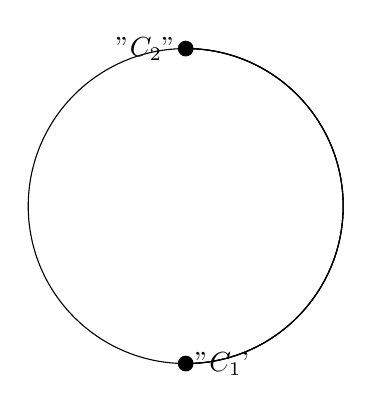
\begin{tikzpicture}[scale=2]
    % Draw the circle
    \draw (0,0) circle (1);
    
    % Mark the points
    \fill (90:1) circle (0.05);
    \fill (-90:1) circle (0.05);
    
    % Add arrows to indicate the direction of the paths
    \draw[->] (90:1) arc (90:-90:1) node[right] {$"C_{1}$'};
    \draw[->] (-90:1) arc (-90:90:1) node[left] {$"C_{2}"$};
\end{tikzpicture}

\end{document}